\documentclass{extbook}[14pt]
\usepackage{multicol, enumerate, enumitem, hyperref, color, soul, setspace, parskip, fancyhdr, amssymb, amsthm, amsmath, latexsym, units, mathtools}
\everymath{\displaystyle}
\usepackage[headsep=0.5cm,headheight=0cm, left=1 in,right= 1 in,top= 1 in,bottom= 1 in]{geometry}
\usepackage{dashrule}  % Package to use the command below to create lines between items
\newcommand{\litem}[1]{\item #1

\rule{\textwidth}{0.4pt}}
\pagestyle{fancy}
\lhead{}
\chead{Answer Key for Progress Quiz 10 Version ALL}
\rhead{}
\lfoot{5170-5105}
\cfoot{}
\rfoot{Summer C 2021}
\begin{document}
\textbf{This key should allow you to understand why you choose the option you did (beyond just getting a question right or wrong). \href{https://xronos.clas.ufl.edu/mac1105spring2020/courseDescriptionAndMisc/Exams/LearningFromResults}{More instructions on how to use this key can be found here}.}

\textbf{If you have a suggestion to make the keys better, \href{https://forms.gle/CZkbZmPbC9XALEE88}{please fill out the short survey here}.}

\textit{Note: This key is auto-generated and may contain issues and/or errors. The keys are reviewed after each exam to ensure grading is done accurately. If there are issues (like duplicate options), they are noted in the offline gradebook. The keys are a work-in-progress to give students as many resources to improve as possible.}

\rule{\textwidth}{0.4pt}

\begin{enumerate}\litem{
Which of the following equations \textit{could} be of the graph presented below?

\begin{center}
    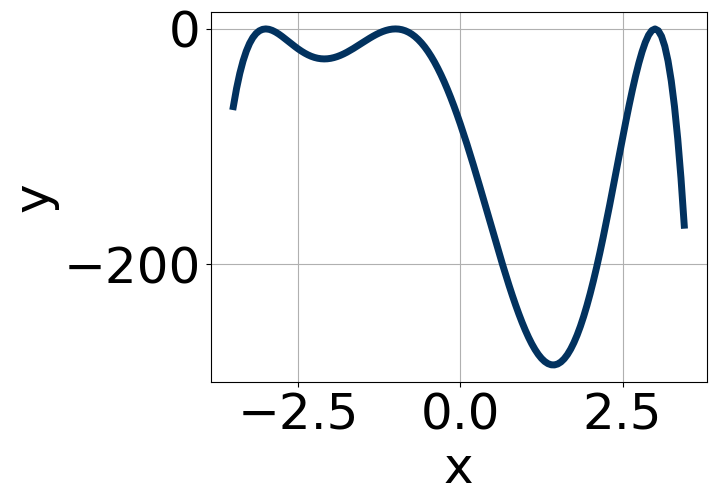
\includegraphics[width=0.5\textwidth]{../Figures/polyGraphToFunctionA.png}
\end{center}


The solution is \( -18(x + 3)^{6} (x + 1)^{4} (x - 3)^{8} \), which is option A.\begin{enumerate}[label=\Alph*.]
\item \( -18(x + 3)^{6} (x + 1)^{4} (x - 3)^{8} \)

* This is the correct option.
\item \( 12(x + 3)^{8} (x + 1)^{4} (x - 3)^{7} \)

The factor $(x - 3)$ should have an even power and the leading coefficient should be the opposite sign.
\item \( -7(x + 3)^{6} (x + 1)^{10} (x - 3)^{7} \)

The factor $(x - 3)$ should have an even power.
\item \( 8(x + 3)^{6} (x + 1)^{6} (x - 3)^{6} \)

This corresponds to the leading coefficient being the opposite value than it should be.
\item \( -12(x + 3)^{10} (x + 1)^{11} (x - 3)^{5} \)

The factors $(x + 1)$ and $(x - 3)$ should both have even powers.
\end{enumerate}

\textbf{General Comment:} General Comments: Draw the x-axis to determine which zeros are touching (and so have even multiplicity) or cross (and have odd multiplicity).
}
\litem{
Describe the end behavior of the polynomial below.
\[ f(x) = -9(x + 8)^{2}(x - 8)^{5}(x - 6)^{2}(x + 6)^{3} \]The solution is the graph below, which is option B.
    \begin{center}
        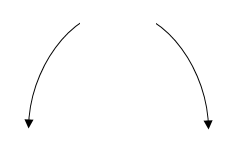
\includegraphics[width=0.3\textwidth]{../Figures/polyEndBehaviorBA.png}
    \end{center}\begin{enumerate}[label=\Alph*.]
\begin{multicols}{2}
\item 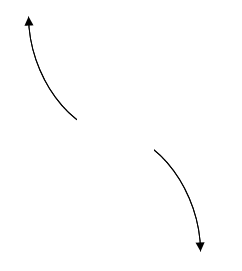
\includegraphics[width = 0.3\textwidth]{../Figures/polyEndBehaviorAA.png}
\item 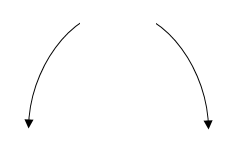
\includegraphics[width = 0.3\textwidth]{../Figures/polyEndBehaviorBA.png}
\item 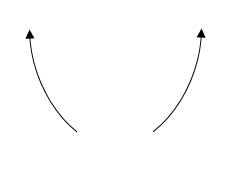
\includegraphics[width = 0.3\textwidth]{../Figures/polyEndBehaviorCA.png}
\item 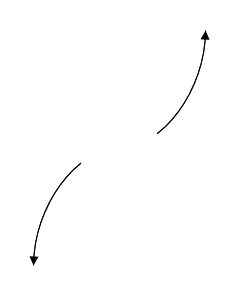
\includegraphics[width = 0.3\textwidth]{../Figures/polyEndBehaviorDA.png}
\end{multicols}\item None of the above.\end{enumerate}
\textbf{General Comment:} Remember that end behavior is determined by the leading coefficient AND whether the \textbf{sum} of the multiplicities is positive or negative.
}
\litem{
Construct the lowest-degree polynomial given the zeros below. Then, choose the intervals that contain the coefficients of the polynomial in the form $x^3+bx^2+cx+d$.
\[ 4 + 3 i \text{ and } 1 \]The solution is \( x^{3} -9 x^{2} +33 x -25 \), which is option C.\begin{enumerate}[label=\Alph*.]
\item \( b \in [1, 2], c \in [-6, -4.35], \text{ and } d \in [3.48, 4.06] \)

$x^{3} + x^{2} -5 x + 4$, which corresponds to multiplying out $(x -4)(x -1)$.
\item \( b \in [1, 2], c \in [-4.24, -2.63], \text{ and } d \in [2.96, 3.37] \)

$x^{3} + x^{2} -4 x + 3$, which corresponds to multiplying out $(x -3)(x -1)$.
\item \( b \in [-17, -7], c \in [31.51, 33.82], \text{ and } d \in [-25.2, -24.86] \)

* $x^{3} -9 x^{2} +33 x -25$, which is the correct option.
\item \( b \in [8, 10], c \in [31.51, 33.82], \text{ and } d \in [24.44, 25.5] \)

$x^{3} +9 x^{2} +33 x + 25$, which corresponds to multiplying out $(x-(4 + 3 i))(x-(4 - 3 i))(x + 1)$.
\item \( \text{None of the above.} \)

This corresponds to making an unanticipated error or not understanding how to use nonreal complex numbers to create the lowest-degree polynomial. If you chose this and are not sure what you did wrong, please contact the coordinator for help.
\end{enumerate}

\textbf{General Comment:} Remember that the conjugate of $a+bi$ is $a-bi$. Since these zeros always come in pairs, we need to multiply out $(x-(4 + 3 i))(x-(4 - 3 i))(x-(1))$.
}
\litem{
Which of the following equations \textit{could} be of the graph presented below?

\begin{center}
    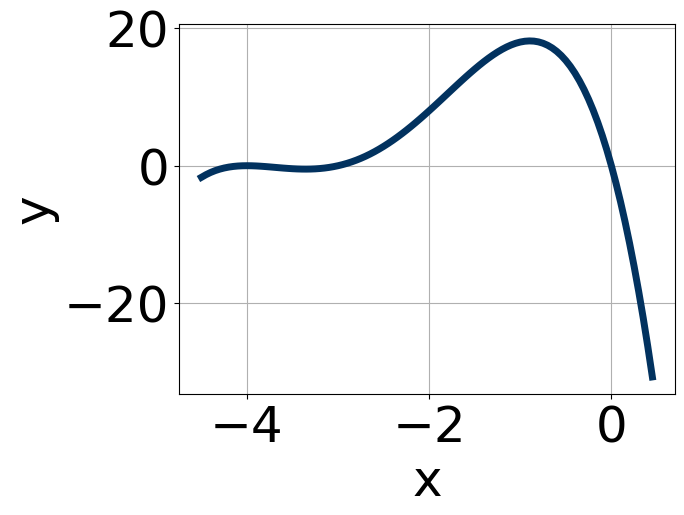
\includegraphics[width=0.5\textwidth]{../Figures/polyGraphToFunctionCopyA.png}
\end{center}


The solution is \( -5x^{5} (x + 4)^{8} (x + 3)^{7} \), which is option A.\begin{enumerate}[label=\Alph*.]
\item \( -5x^{5} (x + 4)^{8} (x + 3)^{7} \)

* This is the correct option.
\item \( -19x^{6} (x + 4)^{6} (x + 3)^{7} \)

The factor $x$ should have an odd power.
\item \( -14x^{10} (x + 4)^{9} (x + 3)^{5} \)

The factor $-4$ should have an even power and the factor $0$ should have an odd power.
\item \( 10x^{11} (x + 4)^{8} (x + 3)^{10} \)

The factor $(x + 3)$ should have an odd power and the leading coefficient should be the opposite sign.
\item \( 19x^{11} (x + 4)^{4} (x + 3)^{7} \)

This corresponds to the leading coefficient being the opposite value than it should be.
\end{enumerate}

\textbf{General Comment:} General Comments: Draw the x-axis to determine which zeros are touching (and so have even multiplicity) or cross (and have odd multiplicity).
}
\litem{
Describe the zero behavior of the zero $x = 8$ of the polynomial below.
\[ f(x) = -9(x - 6)^{9}(x + 6)^{6}(x - 8)^{12}(x + 8)^{9} \]The solution is the graph below, which is option B.
    \begin{center}
        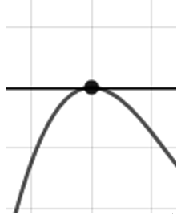
\includegraphics[width=0.3\textwidth]{../Figures/polyZeroBehaviorCopyBA.png}
    \end{center}\begin{enumerate}[label=\Alph*.]
\begin{multicols}{2}
\item 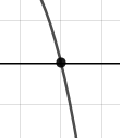
\includegraphics[width = 0.3\textwidth]{../Figures/polyZeroBehaviorCopyAA.png}
\item 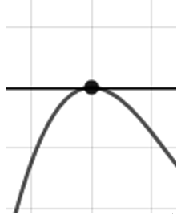
\includegraphics[width = 0.3\textwidth]{../Figures/polyZeroBehaviorCopyBA.png}
\item 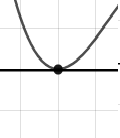
\includegraphics[width = 0.3\textwidth]{../Figures/polyZeroBehaviorCopyCA.png}
\item 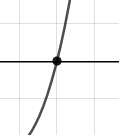
\includegraphics[width = 0.3\textwidth]{../Figures/polyZeroBehaviorCopyDA.png}
\end{multicols}\item None of the above.\end{enumerate}
\textbf{General Comment:} You will need to sketch the entire graph, then zoom in on the zero the question asks about.
}
\litem{
Construct the lowest-degree polynomial given the zeros below. Then, choose the intervals that contain the coefficients of the polynomial in the form $ax^3+bx^2+cx+d$.
\[ \frac{3}{2}, 5, \text{ and } \frac{-4}{3} \]The solution is \( 6x^{3} -31 x^{2} -7 x + 60 \), which is option B.\begin{enumerate}[label=\Alph*.]
\item \( a \in [0, 10], b \in [45, 52], c \in [97, 103], \text{ and } d \in [55, 64] \)

$6x^{3} +47 x^{2} +97 x + 60$, which corresponds to multiplying out $(2x + 3)(x + 5)(3x + 4)$.
\item \( a \in [0, 10], b \in [-34, -27], c \in [-9, -4], \text{ and } d \in [55, 64] \)

* $6x^{3} -31 x^{2} -7 x + 60$, which is the correct option.
\item \( a \in [0, 10], b \in [-34, -27], c \in [-9, -4], \text{ and } d \in [-66, -56] \)

$6x^{3} -31 x^{2} -7 x -60$, which corresponds to multiplying everything correctly except the constant term.
\item \( a \in [0, 10], b \in [26, 37], c \in [-9, -4], \text{ and } d \in [-66, -56] \)

$6x^{3} +31 x^{2} -7 x -60$, which corresponds to multiplying out $(2x + 3)(x + 5)(3x -4)$.
\item \( a \in [0, 10], b \in [-13, -7], c \in [-76, -68], \text{ and } d \in [-66, -56] \)

$6x^{3} -13 x^{2} -73 x -60$, which corresponds to multiplying out $(2x + 3)(x -5)(3x + 4)$.
\end{enumerate}

\textbf{General Comment:} To construct the lowest-degree polynomial, you want to multiply out $(2x -3)(x -5)(3x + 4)$
}
\litem{
Construct the lowest-degree polynomial given the zeros below. Then, choose the intervals that contain the coefficients of the polynomial in the form $x^3+bx^2+cx+d$.
\[ -3 + 2 i \text{ and } 2 \]The solution is \( x^{3} +4 x^{2} +x -26 \), which is option C.\begin{enumerate}[label=\Alph*.]
\item \( b \in [-5.5, -1.2], c \in [-3, 3], \text{ and } d \in [24, 27] \)

$x^{3} -4 x^{2} +x + 26$, which corresponds to multiplying out $(x-(-3 + 2 i))(x-(-3 - 2 i))(x + 2)$.
\item \( b \in [0.7, 1.5], c \in [-6, -3], \text{ and } d \in [0, 9] \)

$x^{3} + x^{2} -4 x + 4$, which corresponds to multiplying out $(x -2)(x -2)$.
\item \( b \in [3.8, 5.3], c \in [-3, 3], \text{ and } d \in [-32, -24] \)

* $x^{3} +4 x^{2} +x -26$, which is the correct option.
\item \( b \in [0.7, 1.5], c \in [-3, 3], \text{ and } d \in [-10, -3] \)

$x^{3} + x^{2} +x -6$, which corresponds to multiplying out $(x + 3)(x -2)$.
\item \( \text{None of the above.} \)

This corresponds to making an unanticipated error or not understanding how to use nonreal complex numbers to create the lowest-degree polynomial. If you chose this and are not sure what you did wrong, please contact the coordinator for help.
\end{enumerate}

\textbf{General Comment:} Remember that the conjugate of $a+bi$ is $a-bi$. Since these zeros always come in pairs, we need to multiply out $(x-(-3 + 2 i))(x-(-3 - 2 i))(x-(2))$.
}
\litem{
Construct the lowest-degree polynomial given the zeros below. Then, choose the intervals that contain the coefficients of the polynomial in the form $ax^3+bx^2+cx+d$.
\[ \frac{-3}{5}, \frac{-7}{2}, \text{ and } \frac{-3}{2} \]The solution is \( 20x^{3} +112 x^{2} +165 x + 63 \), which is option C.\begin{enumerate}[label=\Alph*.]
\item \( a \in [15, 23], b \in [110, 119], c \in [165, 169], \text{ and } d \in [-64, -58] \)

$20x^{3} +112 x^{2} +165 x -63$, which corresponds to multiplying everything correctly except the constant term.
\item \( a \in [15, 23], b \in [-117, -109], c \in [165, 169], \text{ and } d \in [-64, -58] \)

$20x^{3} -112 x^{2} +165 x -63$, which corresponds to multiplying out $(5x -3)(2x -7)(2x -3)$.
\item \( a \in [15, 23], b \in [110, 119], c \in [165, 169], \text{ and } d \in [54, 68] \)

* $20x^{3} +112 x^{2} +165 x + 63$, which is the correct option.
\item \( a \in [15, 23], b \in [-53, -49], c \in [-85, -80], \text{ and } d \in [54, 68] \)

$20x^{3} -52 x^{2} -81 x + 63$, which corresponds to multiplying out $(5x -3)(2x -7)(2x + 3)$.
\item \( a \in [15, 23], b \in [88, 93], c \in [36, 51], \text{ and } d \in [-64, -58] \)

$20x^{3} +88 x^{2} +45 x -63$, which corresponds to multiplying out $(5x -3)(2x + 7)(2x + 3)$.
\end{enumerate}

\textbf{General Comment:} To construct the lowest-degree polynomial, you want to multiply out $(5x + 3)(2x + 7)(2x + 3)$
}
\litem{
Describe the zero behavior of the zero $x = 7$ of the polynomial below.
\[ f(x) = 2(x + 7)^{7}(x - 7)^{10}(x - 3)^{4}(x + 3)^{8} \]The solution is the graph below, which is option C.
    \begin{center}
        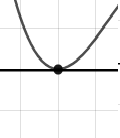
\includegraphics[width=0.3\textwidth]{../Figures/polyZeroBehaviorCA.png}
    \end{center}\begin{enumerate}[label=\Alph*.]
\begin{multicols}{2}
\item 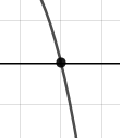
\includegraphics[width = 0.3\textwidth]{../Figures/polyZeroBehaviorAA.png}
\item 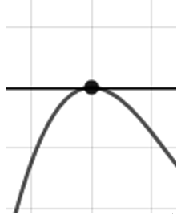
\includegraphics[width = 0.3\textwidth]{../Figures/polyZeroBehaviorBA.png}
\item 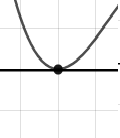
\includegraphics[width = 0.3\textwidth]{../Figures/polyZeroBehaviorCA.png}
\item 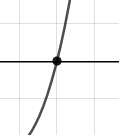
\includegraphics[width = 0.3\textwidth]{../Figures/polyZeroBehaviorDA.png}
\end{multicols}\item None of the above.\end{enumerate}
\textbf{General Comment:} You will need to sketch the entire graph, then zoom in on the zero the question asks about.
}
\litem{
Describe the end behavior of the polynomial below.
\[ f(x) = -3(x + 4)^{3}(x - 4)^{6}(x - 5)^{5}(x + 5)^{7} \]The solution is the graph below, which is option A.
    \begin{center}
        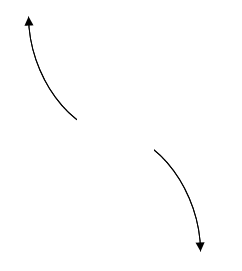
\includegraphics[width=0.3\textwidth]{../Figures/polyEndBehaviorCopyAA.png}
    \end{center}\begin{enumerate}[label=\Alph*.]
\begin{multicols}{2}
\item 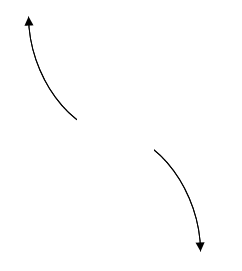
\includegraphics[width = 0.3\textwidth]{../Figures/polyEndBehaviorCopyAA.png}
\item 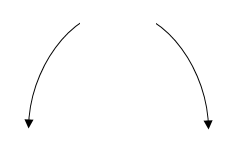
\includegraphics[width = 0.3\textwidth]{../Figures/polyEndBehaviorCopyBA.png}
\item 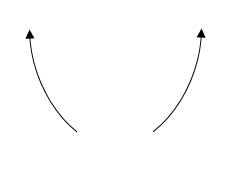
\includegraphics[width = 0.3\textwidth]{../Figures/polyEndBehaviorCopyCA.png}
\item 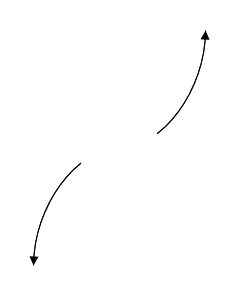
\includegraphics[width = 0.3\textwidth]{../Figures/polyEndBehaviorCopyDA.png}
\end{multicols}\item None of the above.\end{enumerate}
\textbf{General Comment:} Remember that end behavior is determined by the leading coefficient AND whether the \textbf{sum} of the multiplicities is positive or negative.
}
\litem{
Which of the following equations \textit{could} be of the graph presented below?

\begin{center}
    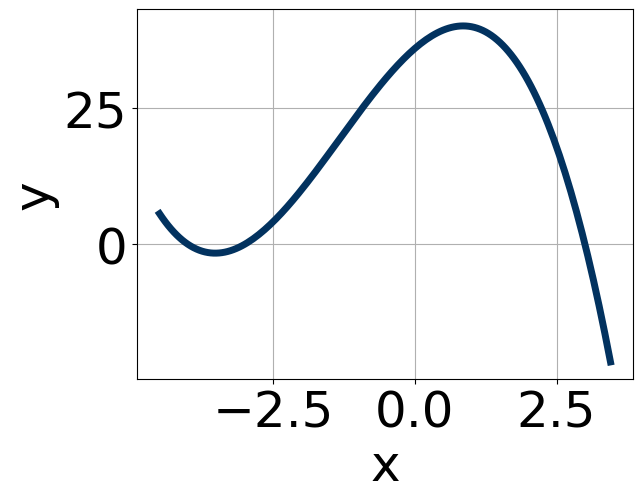
\includegraphics[width=0.5\textwidth]{../Figures/polyGraphToFunctionB.png}
\end{center}


The solution is \( -3(x - 3)^{7} (x + 4)^{9} (x + 3)^{11} \), which is option B.\begin{enumerate}[label=\Alph*.]
\item \( -20(x - 3)^{6} (x + 4)^{11} (x + 3)^{5} \)

The factor $3$ should have been an odd power.
\item \( -3(x - 3)^{7} (x + 4)^{9} (x + 3)^{11} \)

* This is the correct option.
\item \( 6(x - 3)^{4} (x + 4)^{11} (x + 3)^{9} \)

The factor $(x - 3)$ should have an odd power and the leading coefficient should be the opposite sign.
\item \( -3(x - 3)^{4} (x + 4)^{8} (x + 3)^{9} \)

The factors $3$ and $-4$ have have been odd power.
\item \( 18(x - 3)^{5} (x + 4)^{5} (x + 3)^{11} \)

This corresponds to the leading coefficient being the opposite value than it should be.
\end{enumerate}

\textbf{General Comment:} General Comments: Draw the x-axis to determine which zeros are touching (and so have even multiplicity) or cross (and have odd multiplicity).
}
\litem{
Describe the end behavior of the polynomial below.
\[ f(x) = 6(x + 4)^{5}(x - 4)^{6}(x - 3)^{4}(x + 3)^{5} \]The solution is the graph below, which is option C.
    \begin{center}
        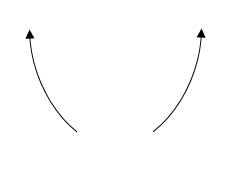
\includegraphics[width=0.3\textwidth]{../Figures/polyEndBehaviorCB.png}
    \end{center}\begin{enumerate}[label=\Alph*.]
\begin{multicols}{2}
\item 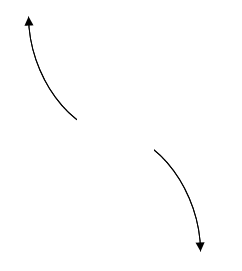
\includegraphics[width = 0.3\textwidth]{../Figures/polyEndBehaviorAB.png}
\item 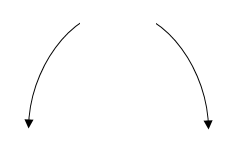
\includegraphics[width = 0.3\textwidth]{../Figures/polyEndBehaviorBB.png}
\item 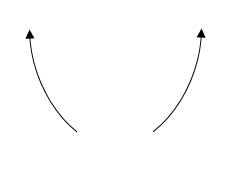
\includegraphics[width = 0.3\textwidth]{../Figures/polyEndBehaviorCB.png}
\item 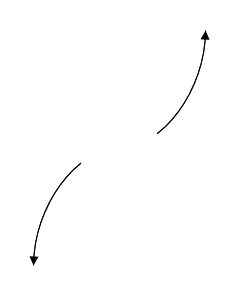
\includegraphics[width = 0.3\textwidth]{../Figures/polyEndBehaviorDB.png}
\end{multicols}\item None of the above.\end{enumerate}
\textbf{General Comment:} Remember that end behavior is determined by the leading coefficient AND whether the \textbf{sum} of the multiplicities is positive or negative.
}
\litem{
Construct the lowest-degree polynomial given the zeros below. Then, choose the intervals that contain the coefficients of the polynomial in the form $x^3+bx^2+cx+d$.
\[ -5 + 5 i \text{ and } -3 \]The solution is \( x^{3} +13 x^{2} +80 x + 150 \), which is option B.\begin{enumerate}[label=\Alph*.]
\item \( b \in [-1, 9], c \in [-8, 1], \text{ and } d \in [-15, -11] \)

$x^{3} + x^{2} -2 x -15$, which corresponds to multiplying out $(x -5)(x + 3)$.
\item \( b \in [11, 16], c \in [80, 82], \text{ and } d \in [147, 158] \)

* $x^{3} +13 x^{2} +80 x + 150$, which is the correct option.
\item \( b \in [-1, 9], c \in [7, 11], \text{ and } d \in [11, 19] \)

$x^{3} + x^{2} +8 x + 15$, which corresponds to multiplying out $(x + 5)(x + 3)$.
\item \( b \in [-19, -12], c \in [80, 82], \text{ and } d \in [-158, -146] \)

$x^{3} -13 x^{2} +80 x -150$, which corresponds to multiplying out $(x-(-5 + 5 i))(x-(-5 - 5 i))(x -3)$.
\item \( \text{None of the above.} \)

This corresponds to making an unanticipated error or not understanding how to use nonreal complex numbers to create the lowest-degree polynomial. If you chose this and are not sure what you did wrong, please contact the coordinator for help.
\end{enumerate}

\textbf{General Comment:} Remember that the conjugate of $a+bi$ is $a-bi$. Since these zeros always come in pairs, we need to multiply out $(x-(-5 + 5 i))(x-(-5 - 5 i))(x-(-3))$.
}
\litem{
Which of the following equations \textit{could} be of the graph presented below?

\begin{center}
    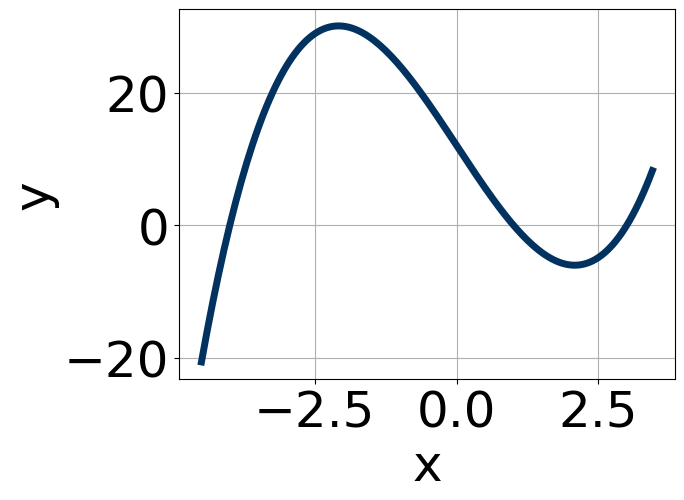
\includegraphics[width=0.5\textwidth]{../Figures/polyGraphToFunctionCopyB.png}
\end{center}


The solution is \( 9(x - 3)^{7} (x + 4)^{11} (x - 1)^{11} \), which is option C.\begin{enumerate}[label=\Alph*.]
\item \( 3(x - 3)^{4} (x + 4)^{8} (x - 1)^{5} \)

The factors $3$ and $-4$ have have been odd power.
\item \( -12(x - 3)^{4} (x + 4)^{5} (x - 1)^{7} \)

The factor $(x - 3)$ should have an odd power and the leading coefficient should be the opposite sign.
\item \( 9(x - 3)^{7} (x + 4)^{11} (x - 1)^{11} \)

* This is the correct option.
\item \( -12(x - 3)^{9} (x + 4)^{11} (x - 1)^{5} \)

This corresponds to the leading coefficient being the opposite value than it should be.
\item \( 10(x - 3)^{6} (x + 4)^{11} (x - 1)^{7} \)

The factor $3$ should have been an odd power.
\end{enumerate}

\textbf{General Comment:} General Comments: Draw the x-axis to determine which zeros are touching (and so have even multiplicity) or cross (and have odd multiplicity).
}
\litem{
Describe the zero behavior of the zero $x = -8$ of the polynomial below.
\[ f(x) = 9(x + 2)^{11}(x - 2)^{7}(x + 8)^{7}(x - 8)^{6} \]The solution is the graph below, which is option D.
    \begin{center}
        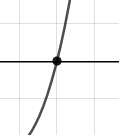
\includegraphics[width=0.3\textwidth]{../Figures/polyZeroBehaviorCopyDB.png}
    \end{center}\begin{enumerate}[label=\Alph*.]
\begin{multicols}{2}
\item 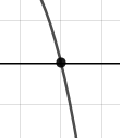
\includegraphics[width = 0.3\textwidth]{../Figures/polyZeroBehaviorCopyAB.png}
\item 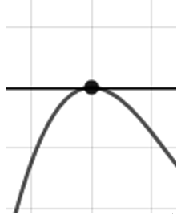
\includegraphics[width = 0.3\textwidth]{../Figures/polyZeroBehaviorCopyBB.png}
\item 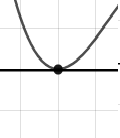
\includegraphics[width = 0.3\textwidth]{../Figures/polyZeroBehaviorCopyCB.png}
\item 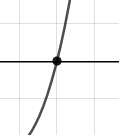
\includegraphics[width = 0.3\textwidth]{../Figures/polyZeroBehaviorCopyDB.png}
\end{multicols}\item None of the above.\end{enumerate}
\textbf{General Comment:} You will need to sketch the entire graph, then zoom in on the zero the question asks about.
}
\litem{
Construct the lowest-degree polynomial given the zeros below. Then, choose the intervals that contain the coefficients of the polynomial in the form $ax^3+bx^2+cx+d$.
\[ \frac{5}{2}, \frac{-1}{3}, \text{ and } \frac{-2}{3} \]The solution is \( 18x^{3} -27 x^{2} -41 x -10 \), which is option B.\begin{enumerate}[label=\Alph*.]
\item \( a \in [17, 23], b \in [19, 28], c \in [-45, -36], \text{ and } d \in [8, 11] \)

$18x^{3} +27 x^{2} -41 x + 10$, which corresponds to multiplying out $(2x + 5)(3x -1)(3x -2)$.
\item \( a \in [17, 23], b \in [-27, -24], c \in [-45, -36], \text{ and } d \in [-17, -9] \)

* $18x^{3} -27 x^{2} -41 x -10$, which is the correct option.
\item \( a \in [17, 23], b \in [50, 54], c \in [3, 12], \text{ and } d \in [-17, -9] \)

$18x^{3} +51 x^{2} +11 x -10$, which corresponds to multiplying out $(2x + 5)(3x -1)(3x + 2)$.
\item \( a \in [17, 23], b \in [58, 75], c \in [44, 53], \text{ and } d \in [8, 11] \)

$18x^{3} +63 x^{2} +49 x + 10$, which corresponds to multiplying out $(2x + 5)(3x + 1)(3x + 2)$.
\item \( a \in [17, 23], b \in [-27, -24], c \in [-45, -36], \text{ and } d \in [8, 11] \)

$18x^{3} -27 x^{2} -41 x + 10$, which corresponds to multiplying everything correctly except the constant term.
\end{enumerate}

\textbf{General Comment:} To construct the lowest-degree polynomial, you want to multiply out $(2x -5)(3x + 1)(3x + 2)$
}
\litem{
Construct the lowest-degree polynomial given the zeros below. Then, choose the intervals that contain the coefficients of the polynomial in the form $x^3+bx^2+cx+d$.
\[ 4 + 5 i \text{ and } -2 \]The solution is \( x^{3} -6 x^{2} +25 x + 82 \), which is option D.\begin{enumerate}[label=\Alph*.]
\item \( b \in [1, 3], c \in [-4.5, -2.7], \text{ and } d \in [-10.1, -9.4] \)

$x^{3} + x^{2} -3 x -10$, which corresponds to multiplying out $(x -5)(x + 2)$.
\item \( b \in [1, 3], c \in [-2.53, -1.56], \text{ and } d \in [-8.9, -6.6] \)

$x^{3} + x^{2} -2 x -8$, which corresponds to multiplying out $(x -4)(x + 2)$.
\item \( b \in [6, 11], c \in [22.96, 25.33], \text{ and } d \in [-83.9, -75.9] \)

$x^{3} +6 x^{2} +25 x -82$, which corresponds to multiplying out $(x-(4 + 5 i))(x-(4 - 5 i))(x -2)$.
\item \( b \in [-7, -3], c \in [22.96, 25.33], \text{ and } d \in [80.5, 82.2] \)

* $x^{3} -6 x^{2} +25 x + 82$, which is the correct option.
\item \( \text{None of the above.} \)

This corresponds to making an unanticipated error or not understanding how to use nonreal complex numbers to create the lowest-degree polynomial. If you chose this and are not sure what you did wrong, please contact the coordinator for help.
\end{enumerate}

\textbf{General Comment:} Remember that the conjugate of $a+bi$ is $a-bi$. Since these zeros always come in pairs, we need to multiply out $(x-(4 + 5 i))(x-(4 - 5 i))(x-(-2))$.
}
\litem{
Construct the lowest-degree polynomial given the zeros below. Then, choose the intervals that contain the coefficients of the polynomial in the form $ax^3+bx^2+cx+d$.
\[ \frac{7}{5}, \frac{-1}{4}, \text{ and } \frac{2}{5} \]The solution is \( 100x^{3} -155 x^{2} +11 x + 14 \), which is option C.\begin{enumerate}[label=\Alph*.]
\item \( a \in [97, 103], b \in [75, 77], c \in [-81, -77], \text{ and } d \in [6, 19] \)

$100x^{3} +75 x^{2} -81 x + 14$, which corresponds to multiplying out $(5x + 7)(4x -1)(5x -2)$.
\item \( a \in [97, 103], b \in [-163, -151], c \in [5, 14], \text{ and } d \in [-14, -13] \)

$100x^{3} -155 x^{2} +11 x -14$, which corresponds to multiplying everything correctly except the constant term.
\item \( a \in [97, 103], b \in [-163, -151], c \in [5, 14], \text{ and } d \in [6, 19] \)

* $100x^{3} -155 x^{2} +11 x + 14$, which is the correct option.
\item \( a \in [97, 103], b \in [147, 156], c \in [5, 14], \text{ and } d \in [-14, -13] \)

$100x^{3} +155 x^{2} +11 x -14$, which corresponds to multiplying out $(5x + 7)(4x -1)(5x + 2)$.
\item \( a \in [97, 103], b \in [119, 127], c \in [-37, -25], \text{ and } d \in [-14, -13] \)

$100x^{3} +125 x^{2} -31 x -14$, which corresponds to multiplying out $(5x + 7)(4x + 1)(5x -2)$.
\end{enumerate}

\textbf{General Comment:} To construct the lowest-degree polynomial, you want to multiply out $(5x -7)(4x + 1)(5x -2)$
}
\litem{
Describe the zero behavior of the zero $x = -6$ of the polynomial below.
\[ f(x) = 9(x - 6)^{5}(x + 6)^{10}(x - 9)^{7}(x + 9)^{11} \]The solution is the graph below, which is option C.
    \begin{center}
        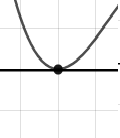
\includegraphics[width=0.3\textwidth]{../Figures/polyZeroBehaviorCB.png}
    \end{center}\begin{enumerate}[label=\Alph*.]
\begin{multicols}{2}
\item 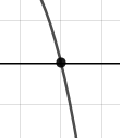
\includegraphics[width = 0.3\textwidth]{../Figures/polyZeroBehaviorAB.png}
\item 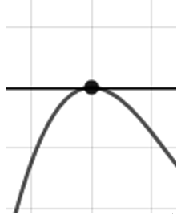
\includegraphics[width = 0.3\textwidth]{../Figures/polyZeroBehaviorBB.png}
\item 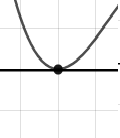
\includegraphics[width = 0.3\textwidth]{../Figures/polyZeroBehaviorCB.png}
\item 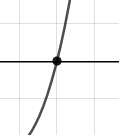
\includegraphics[width = 0.3\textwidth]{../Figures/polyZeroBehaviorDB.png}
\end{multicols}\item None of the above.\end{enumerate}
\textbf{General Comment:} You will need to sketch the entire graph, then zoom in on the zero the question asks about.
}
\litem{
Describe the end behavior of the polynomial below.
\[ f(x) = -8(x - 2)^{4}(x + 2)^{5}(x + 9)^{5}(x - 9)^{6} \]The solution is the graph below, which is option B.
    \begin{center}
        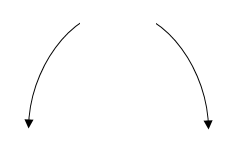
\includegraphics[width=0.3\textwidth]{../Figures/polyEndBehaviorCopyBB.png}
    \end{center}\begin{enumerate}[label=\Alph*.]
\begin{multicols}{2}
\item 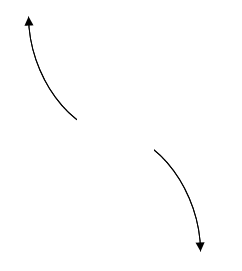
\includegraphics[width = 0.3\textwidth]{../Figures/polyEndBehaviorCopyAB.png}
\item 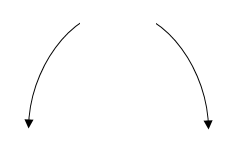
\includegraphics[width = 0.3\textwidth]{../Figures/polyEndBehaviorCopyBB.png}
\item 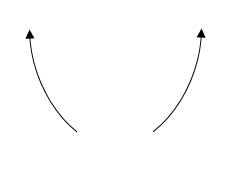
\includegraphics[width = 0.3\textwidth]{../Figures/polyEndBehaviorCopyCB.png}
\item 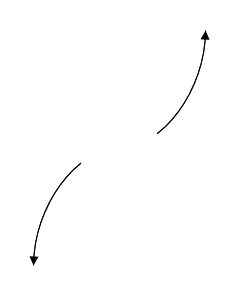
\includegraphics[width = 0.3\textwidth]{../Figures/polyEndBehaviorCopyDB.png}
\end{multicols}\item None of the above.\end{enumerate}
\textbf{General Comment:} Remember that end behavior is determined by the leading coefficient AND whether the \textbf{sum} of the multiplicities is positive or negative.
}
\litem{
Which of the following equations \textit{could} be of the graph presented below?

\begin{center}
    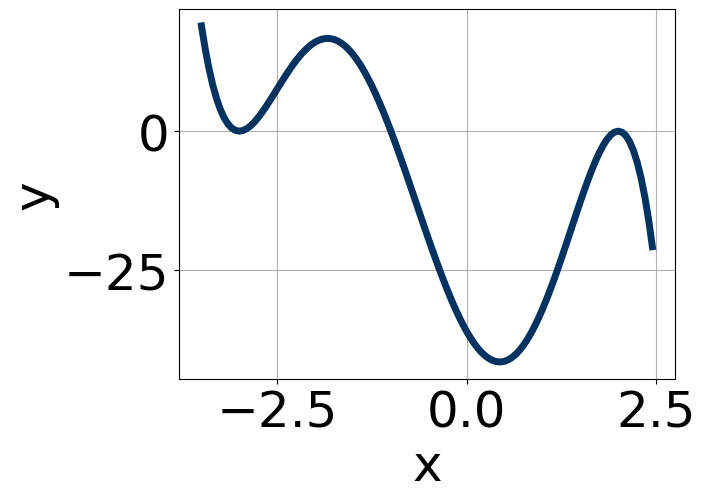
\includegraphics[width=0.5\textwidth]{../Figures/polyGraphToFunctionC.png}
\end{center}


The solution is \( -18(x - 2)^{10} (x + 3)^{6} (x + 1)^{11} \), which is option B.\begin{enumerate}[label=\Alph*.]
\item \( 19(x - 2)^{10} (x + 3)^{6} (x + 1)^{8} \)

The factor $(x + 1)$ should have an odd power and the leading coefficient should be the opposite sign.
\item \( -18(x - 2)^{10} (x + 3)^{6} (x + 1)^{11} \)

* This is the correct option.
\item \( -19(x - 2)^{8} (x + 3)^{9} (x + 1)^{10} \)

The factor $(x + 3)$ should have an even power and the factor $(x + 1)$ should have an odd power.
\item \( 13(x - 2)^{10} (x + 3)^{10} (x + 1)^{5} \)

This corresponds to the leading coefficient being the opposite value than it should be.
\item \( -4(x - 2)^{10} (x + 3)^{5} (x + 1)^{5} \)

The factor $(x + 3)$ should have an even power.
\end{enumerate}

\textbf{General Comment:} General Comments: Draw the x-axis to determine which zeros are touching (and so have even multiplicity) or cross (and have odd multiplicity).
}
\litem{
Describe the end behavior of the polynomial below.
\[ f(x) = 4(x + 6)^{4}(x - 6)^{9}(x + 9)^{3}(x - 9)^{3} \]The solution is the graph below, which is option D.
    \begin{center}
        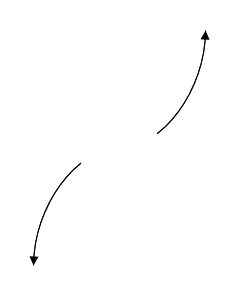
\includegraphics[width=0.3\textwidth]{../Figures/polyEndBehaviorDC.png}
    \end{center}\begin{enumerate}[label=\Alph*.]
\begin{multicols}{2}
\item 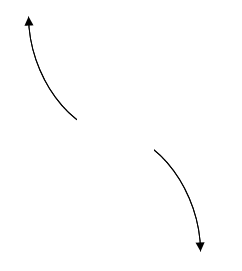
\includegraphics[width = 0.3\textwidth]{../Figures/polyEndBehaviorAC.png}
\item 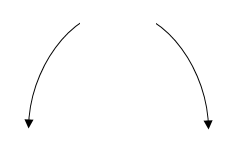
\includegraphics[width = 0.3\textwidth]{../Figures/polyEndBehaviorBC.png}
\item 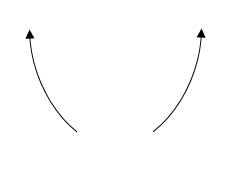
\includegraphics[width = 0.3\textwidth]{../Figures/polyEndBehaviorCC.png}
\item 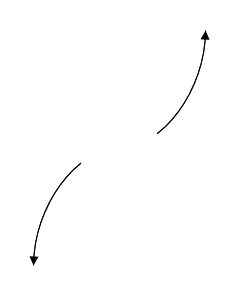
\includegraphics[width = 0.3\textwidth]{../Figures/polyEndBehaviorDC.png}
\end{multicols}\item None of the above.\end{enumerate}
\textbf{General Comment:} Remember that end behavior is determined by the leading coefficient AND whether the \textbf{sum} of the multiplicities is positive or negative.
}
\litem{
Construct the lowest-degree polynomial given the zeros below. Then, choose the intervals that contain the coefficients of the polynomial in the form $x^3+bx^2+cx+d$.
\[ -3 - 5 i \text{ and } -4 \]The solution is \( x^{3} +10 x^{2} +58 x + 136 \), which is option D.\begin{enumerate}[label=\Alph*.]
\item \( b \in [-1, 5], c \in [8, 9.7], \text{ and } d \in [16, 22] \)

$x^{3} + x^{2} +9 x + 20$, which corresponds to multiplying out $(x + 5)(x + 4)$.
\item \( b \in [-1, 5], c \in [6.7, 8.6], \text{ and } d \in [10, 14] \)

$x^{3} + x^{2} +7 x + 12$, which corresponds to multiplying out $(x + 3)(x + 4)$.
\item \( b \in [-15, -8], c \in [56.1, 58.3], \text{ and } d \in [-143, -134] \)

$x^{3} -10 x^{2} +58 x -136$, which corresponds to multiplying out $(x-(-3 - 5 i))(x-(-3 + 5 i))(x -4)$.
\item \( b \in [6, 14], c \in [56.1, 58.3], \text{ and } d \in [130, 141] \)

* $x^{3} +10 x^{2} +58 x + 136$, which is the correct option.
\item \( \text{None of the above.} \)

This corresponds to making an unanticipated error or not understanding how to use nonreal complex numbers to create the lowest-degree polynomial. If you chose this and are not sure what you did wrong, please contact the coordinator for help.
\end{enumerate}

\textbf{General Comment:} Remember that the conjugate of $a+bi$ is $a-bi$. Since these zeros always come in pairs, we need to multiply out $(x-(-3 - 5 i))(x-(-3 + 5 i))(x-(-4))$.
}
\litem{
Which of the following equations \textit{could} be of the graph presented below?

\begin{center}
    \includegraphics[width=0.5\textwidth]{../Figures/polyGraphToFunctionCopyC.png}
\end{center}


The solution is \( -2(x + 2)^{9} (x + 3)^{11} (x - 3)^{5} \), which is option D.\begin{enumerate}[label=\Alph*.]
\item \( 7(x + 2)^{6} (x + 3)^{11} (x - 3)^{7} \)

The factor $(x + 2)$ should have an odd power and the leading coefficient should be the opposite sign.
\item \( -10(x + 2)^{10} (x + 3)^{9} (x - 3)^{9} \)

The factor $-2$ should have been an odd power.
\item \( 11(x + 2)^{9} (x + 3)^{9} (x - 3)^{9} \)

This corresponds to the leading coefficient being the opposite value than it should be.
\item \( -2(x + 2)^{9} (x + 3)^{11} (x - 3)^{5} \)

* This is the correct option.
\item \( -5(x + 2)^{4} (x + 3)^{8} (x - 3)^{9} \)

The factors $-2$ and $-3$ have have been odd power.
\end{enumerate}

\textbf{General Comment:} General Comments: Draw the x-axis to determine which zeros are touching (and so have even multiplicity) or cross (and have odd multiplicity).
}
\litem{
Describe the zero behavior of the zero $x = -6$ of the polynomial below.
\[ f(x) = -9(x - 6)^{9}(x + 6)^{10}(x + 2)^{9}(x - 2)^{12} \]The solution is the graph below, which is option B.
    \begin{center}
        \includegraphics[width=0.3\textwidth]{../Figures/polyZeroBehaviorCopyBC.png}
    \end{center}\begin{enumerate}[label=\Alph*.]
\begin{multicols}{2}
\item \includegraphics[width = 0.3\textwidth]{../Figures/polyZeroBehaviorCopyAC.png}
\item \includegraphics[width = 0.3\textwidth]{../Figures/polyZeroBehaviorCopyBC.png}
\item \includegraphics[width = 0.3\textwidth]{../Figures/polyZeroBehaviorCopyCC.png}
\item \includegraphics[width = 0.3\textwidth]{../Figures/polyZeroBehaviorCopyDC.png}
\end{multicols}\item None of the above.\end{enumerate}
\textbf{General Comment:} You will need to sketch the entire graph, then zoom in on the zero the question asks about.
}
\litem{
Construct the lowest-degree polynomial given the zeros below. Then, choose the intervals that contain the coefficients of the polynomial in the form $ax^3+bx^2+cx+d$.
\[ -2, \frac{-7}{3}, \text{ and } \frac{3}{2} \]The solution is \( 6x^{3} +17 x^{2} -11 x -42 \), which is option E.\begin{enumerate}[label=\Alph*.]
\item \( a \in [5, 11], b \in [16, 20], c \in [-14, -9], \text{ and } d \in [40, 47] \)

$6x^{3} +17 x^{2} -11 x + 42$, which corresponds to multiplying everything correctly except the constant term.
\item \( a \in [5, 11], b \in [-12, -2], c \in [-33, -27], \text{ and } d \in [40, 47] \)

$6x^{3} -7 x^{2} -31 x + 42$, which corresponds to multiplying out $(x -2)(3x + 7)(2x -3)$.
\item \( a \in [5, 11], b \in [-43, -32], c \in [63, 68], \text{ and } d \in [-47, -37] \)

$6x^{3} -35 x^{2} +67 x -42$, which corresponds to multiplying out $(x -2)(3x -7)(2x -3)$.
\item \( a \in [5, 11], b \in [-21, -14], c \in [-14, -9], \text{ and } d \in [40, 47] \)

$6x^{3} -17 x^{2} -11 x + 42$, which corresponds to multiplying out $(x -2)(3x -7)(2x + 3)$.
\item \( a \in [5, 11], b \in [16, 20], c \in [-14, -9], \text{ and } d \in [-47, -37] \)

* $6x^{3} +17 x^{2} -11 x -42$, which is the correct option.
\end{enumerate}

\textbf{General Comment:} To construct the lowest-degree polynomial, you want to multiply out $(x + 2)(3x + 7)(2x -3)$
}
\litem{
Construct the lowest-degree polynomial given the zeros below. Then, choose the intervals that contain the coefficients of the polynomial in the form $x^3+bx^2+cx+d$.
\[ -4 - 3 i \text{ and } -3 \]The solution is \( x^{3} +11 x^{2} +49 x + 75 \), which is option A.\begin{enumerate}[label=\Alph*.]
\item \( b \in [11, 19], c \in [48.36, 49.78], \text{ and } d \in [72.6, 77.1] \)

* $x^{3} +11 x^{2} +49 x + 75$, which is the correct option.
\item \( b \in [0, 7], c \in [4.02, 6.83], \text{ and } d \in [7.9, 9.5] \)

$x^{3} + x^{2} +6 x + 9$, which corresponds to multiplying out $(x + 3)(x + 3)$.
\item \( b \in [0, 7], c \in [6.29, 9.06], \text{ and } d \in [11.8, 14.7] \)

$x^{3} + x^{2} +7 x + 12$, which corresponds to multiplying out $(x + 4)(x + 3)$.
\item \( b \in [-16, -10], c \in [48.36, 49.78], \text{ and } d \in [-76, -71.8] \)

$x^{3} -11 x^{2} +49 x -75$, which corresponds to multiplying out $(x-(-4 - 3 i))(x-(-4 + 3 i))(x -3)$.
\item \( \text{None of the above.} \)

This corresponds to making an unanticipated error or not understanding how to use nonreal complex numbers to create the lowest-degree polynomial. If you chose this and are not sure what you did wrong, please contact the coordinator for help.
\end{enumerate}

\textbf{General Comment:} Remember that the conjugate of $a+bi$ is $a-bi$. Since these zeros always come in pairs, we need to multiply out $(x-(-4 - 3 i))(x-(-4 + 3 i))(x-(-3))$.
}
\litem{
Construct the lowest-degree polynomial given the zeros below. Then, choose the intervals that contain the coefficients of the polynomial in the form $ax^3+bx^2+cx+d$.
\[ \frac{-7}{5}, \frac{-1}{4}, \text{ and } \frac{3}{5} \]The solution is \( 100x^{3} +105 x^{2} -64 x -21 \), which is option E.\begin{enumerate}[label=\Alph*.]
\item \( a \in [100, 104], b \in [-230, -224], c \in [129, 136], \text{ and } d \in [-21, -15] \)

$100x^{3} -225 x^{2} +134 x -21$, which corresponds to multiplying out $(5x -7)(4x -1)(5x -3)$.
\item \( a \in [100, 104], b \in [-177, -171], c \in [30, 38], \text{ and } d \in [20, 32] \)

$100x^{3} -175 x^{2} +34 x + 21$, which corresponds to multiplying out $(5x -7)(4x + 1)(5x -3)$.
\item \( a \in [100, 104], b \in [-112, -104], c \in [-65, -60], \text{ and } d \in [20, 32] \)

$100x^{3} -105 x^{2} -64 x + 21$, which corresponds to multiplying out $(5x -7)(4x -1)(5x + 3)$.
\item \( a \in [100, 104], b \in [103, 115], c \in [-65, -60], \text{ and } d \in [20, 32] \)

$100x^{3} +105 x^{2} -64 x + 21$, which corresponds to multiplying everything correctly except the constant term.
\item \( a \in [100, 104], b \in [103, 115], c \in [-65, -60], \text{ and } d \in [-21, -15] \)

* $100x^{3} +105 x^{2} -64 x -21$, which is the correct option.
\end{enumerate}

\textbf{General Comment:} To construct the lowest-degree polynomial, you want to multiply out $(5x + 7)(4x + 1)(5x -3)$
}
\litem{
Describe the zero behavior of the zero $x = 7$ of the polynomial below.
\[ f(x) = -7(x - 3)^{11}(x + 3)^{9}(x - 7)^{14}(x + 7)^{9} \]The solution is the graph below, which is option B.
    \begin{center}
        \includegraphics[width=0.3\textwidth]{../Figures/polyZeroBehaviorBC.png}
    \end{center}\begin{enumerate}[label=\Alph*.]
\begin{multicols}{2}
\item \includegraphics[width = 0.3\textwidth]{../Figures/polyZeroBehaviorAC.png}
\item \includegraphics[width = 0.3\textwidth]{../Figures/polyZeroBehaviorBC.png}
\item \includegraphics[width = 0.3\textwidth]{../Figures/polyZeroBehaviorCC.png}
\item \includegraphics[width = 0.3\textwidth]{../Figures/polyZeroBehaviorDC.png}
\end{multicols}\item None of the above.\end{enumerate}
\textbf{General Comment:} You will need to sketch the entire graph, then zoom in on the zero the question asks about.
}
\litem{
Describe the end behavior of the polynomial below.
\[ f(x) = -3(x + 9)^{5}(x - 9)^{8}(x - 3)^{2}(x + 3)^{3} \]The solution is the graph below, which is option B.
    \begin{center}
        \includegraphics[width=0.3\textwidth]{../Figures/polyEndBehaviorCopyBC.png}
    \end{center}\begin{enumerate}[label=\Alph*.]
\begin{multicols}{2}
\item \includegraphics[width = 0.3\textwidth]{../Figures/polyEndBehaviorCopyAC.png}
\item \includegraphics[width = 0.3\textwidth]{../Figures/polyEndBehaviorCopyBC.png}
\item \includegraphics[width = 0.3\textwidth]{../Figures/polyEndBehaviorCopyCC.png}
\item \includegraphics[width = 0.3\textwidth]{../Figures/polyEndBehaviorCopyDC.png}
\end{multicols}\item None of the above.\end{enumerate}
\textbf{General Comment:} Remember that end behavior is determined by the leading coefficient AND whether the \textbf{sum} of the multiplicities is positive or negative.
}
\end{enumerate}

\end{document}